\subsection{Horizontal Translation}

Here the effects of horizontal translation on the network performance will be presented. \Fig~\ref{fig:acc_ht_wu} shows he alteration graphs for both networks.

For this alteration, the degradation is symmetric for both networks. In this case, the accuracy of the BNN, as shown in \Fig~\ref{fig:ht_acc_wu_bnn}, degrades less than that of the standard NN, shown in \Fig~\ref{fig:brightness_ann}. However, it is evident that both networks are fragile against horizontal translation. As soon as we deviate from the nominal conditions, the accuracy drops significantly.

\begin{figure}[h]
	\centering
	\begin{subfigure}{.5\textwidth}
		\centering
		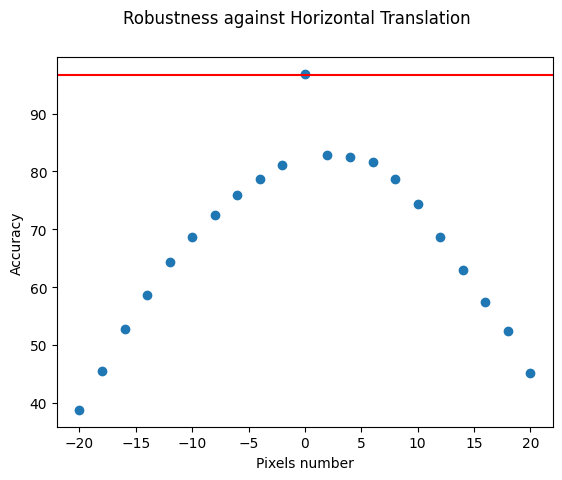
\includegraphics[width=0.9\linewidth]{ImageFiles/EvalBNN/HT/WU/acc}
		\caption{BNN}
		\label{fig:ht_acc_wu_bnn}
	\end{subfigure}%
	\begin{subfigure}{.5\textwidth}
		\centering
		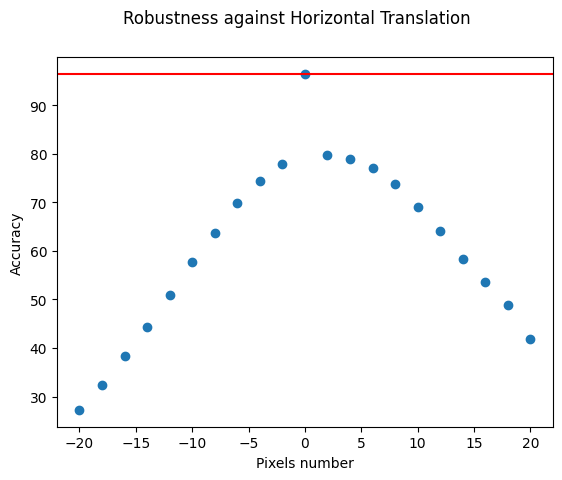
\includegraphics[width=0.9\linewidth]{ImageFiles/EvalANN/horiz_trans_ann}
		\caption{Standard NN}
		\label{fig:horiz_trans_ann}
	\end{subfigure}
	\caption{Accuracy trend for horizontal translation}
	\label{fig:acc_ht_wu}
\end{figure}

The observations made so far are confirmed for the computation of the robustness, which results $0.8563$ for the BNN and $0.8103$ for the standard NN.

Both uncertainties, aleatoric in \Fig~\ref{fig:ht_aleatoric} and epistemic in \Fig~\ref{fig:ht_epistemic}, reflects the degradation seen in the accuracy.

\begin{figure}[h]
	\centering
	\begin{subfigure}{.5\textwidth}
		\centering
		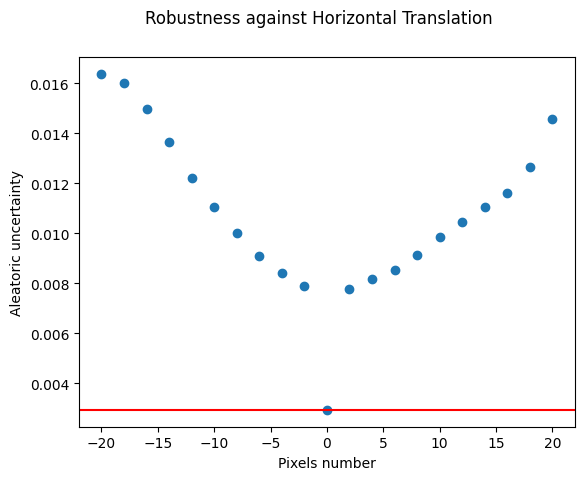
\includegraphics[width=0.9\linewidth]{ImageFiles/EvalBNN/HT/aleatoric}
		\caption{Aleatoric uncertainty}
		\label{fig:ht_aleatoric}
	\end{subfigure}%
	\begin{subfigure}{.5\textwidth}
		\centering
		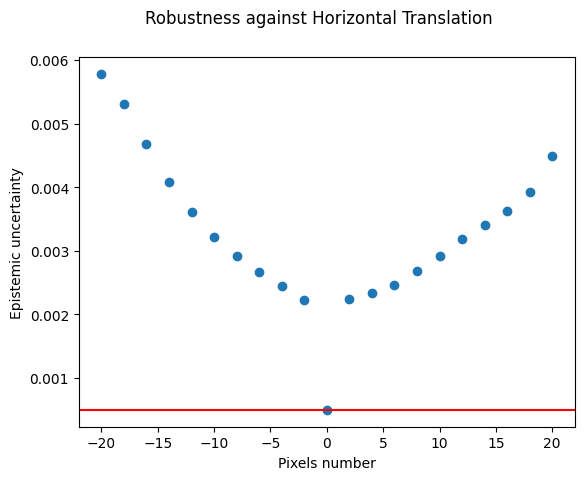
\includegraphics[width=0.9\linewidth]{ImageFiles/EvalBNN/HT/epistemic}
		\caption{Epistemic uncertainty}
		\label{fig:ht_epistemic}
	\end{subfigure}
	\caption{Uncertainty trend for horizontal translation}
	\label{fig:ht_uncertainty}
\end{figure}

This behavior is due to the network architecture. One of the limitations of MLPs is their inability to handle translation and grid data efficiently. This issue can be easily addressed with CNNs) In this analysis, we observe how BNNs extend standard NNs, but they still keep their structural limitations.

\vspace{0.3cm}
\textbf{Classification using aleatoric uncertainty}
\vspace{0.1cm}

The use of aleatoric uncertainty in the classification mitigates the degradation in accuracy, as observed in \Fig~\ref{fig:ht_au_acc}. However, it also leads to a substantial increase in the unknown ratio, as shown in \Fig~\ref{fig:ht_au_unkn}, reaching very high levels. This trade-off is further highlighted in \Fig~\ref{fig:ht_au_eff}, which illustrates the degradation in effectiveness.

\begin{figure}[h]
	\centering
	\begin{subfigure}{.33\textwidth}
		\centering
		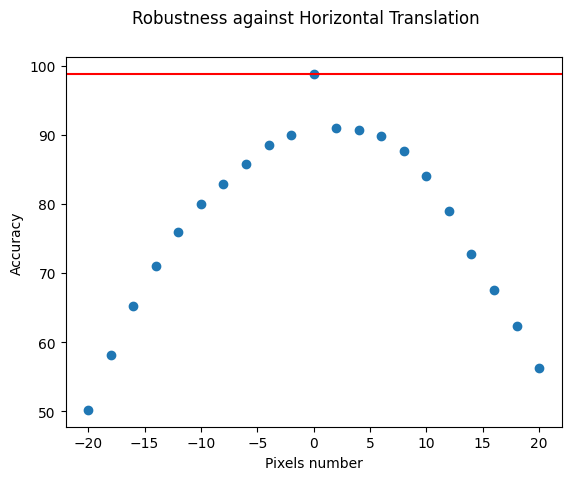
\includegraphics[width=0.9\linewidth]{ImageFiles/EvalBNN/HT/AU/acc}
		\caption{Accuracy using aleatoric \\ uncertainty}
		\label{fig:ht_au_acc}
	\end{subfigure}%
	\begin{subfigure}{.33\textwidth}
		\centering
		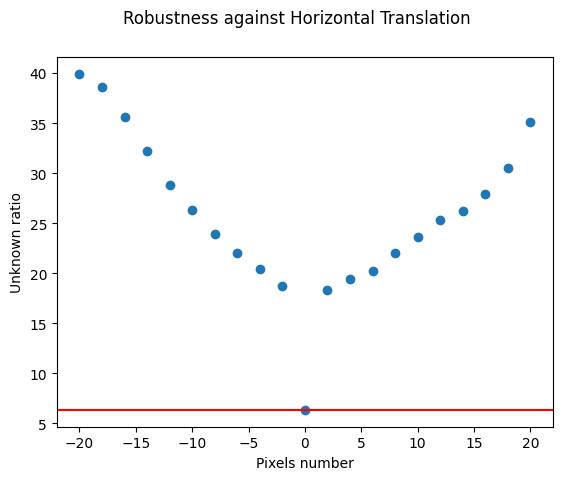
\includegraphics[width=0.9\linewidth]{ImageFiles/EvalBNN/HT/AU/unkn}
		\caption{Unknown ratio using aleatoric uncertainty}
		\label{fig:ht_au_unkn}
	\end{subfigure}%
	\begin{subfigure}{.33\textwidth}
		\centering
		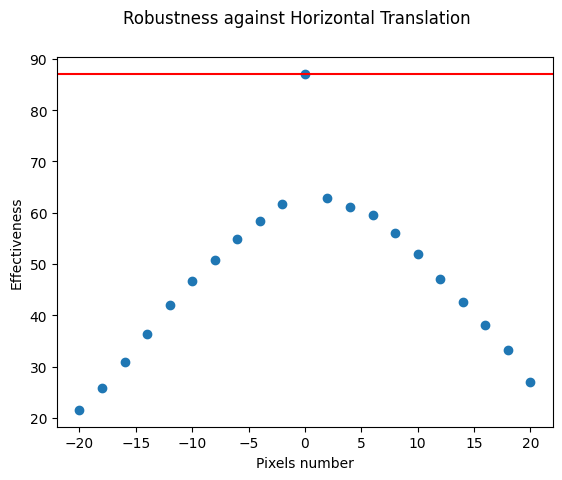
\includegraphics[width=0.9\linewidth]{ImageFiles/EvalBNN/HT/AU/eff}
		\caption{Effectiveness using aleatoric uncertainty}
		\label{fig:ht_au_eff}
	\end{subfigure}
	\caption{Robustness graph for horizontal translation when aleatoric uncertainty is employed in the classification}
	\label{fig:ht_au}
\end{figure}

\Tab~\ref{table:rob_ht_au} indicates that the robustness in terms of accuracy increases, but the augmented robustness is very low due to the high unknown ratio reached.

\begin{table}[h]
	\centering
	\begin{tabular}{|| l | l ||} 
		\hline
		\textbf{Parameter} & \textbf{Value} \\
		\hline
		\hline
		$rob_{HorizontalTranslation}$ & $0.8985$ \\
		$robInd_{HorizontalTranslation}$ & $0.8993$ \\
		$robAug_{HorizontalTranslation}$ & $0.7791$ \\	
		\hline
	\end{tabular}	
	\caption{Robustness metrics for the horizontal translation when the aleatoric uncertainty is employed}
	\label{table:rob_ht_au}
\end{table}

\vspace{0.3cm}
\textbf{Classification using epistemic uncertainty}
\vspace{0.1cm}

The same analysis is conducted for the epistemic uncertainty and the results are shown in \Fig~\ref{fig:ht_eu}. The trends observed are the same as in the previous case.

\begin{figure}[h]
	\centering
	\begin{subfigure}{.33\textwidth}
		\centering
		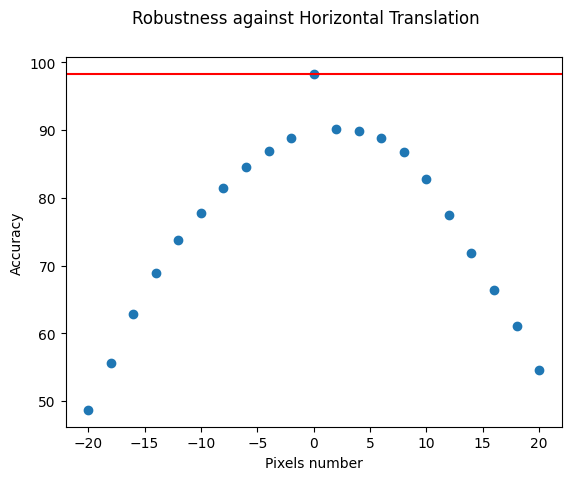
\includegraphics[width=0.9\linewidth]{ImageFiles/EvalBNN/HT/EU/acc}
		\caption{Accuracy using epistemic \\ uncertainty}
		\label{fig:ht_eu_acc}
	\end{subfigure}%
	\begin{subfigure}{.33\textwidth}
		\centering
		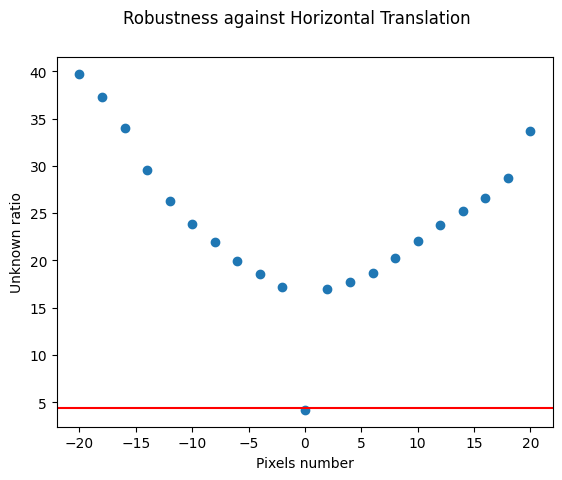
\includegraphics[width=0.9\linewidth]{ImageFiles/EvalBNN/HT/EU/unkn}
		\caption{Unknown ratio using \\ epistemic uncertainty}
		\label{fig:ht_eu_unkn}
	\end{subfigure}%
	\begin{subfigure}{.33\textwidth}
		\centering
		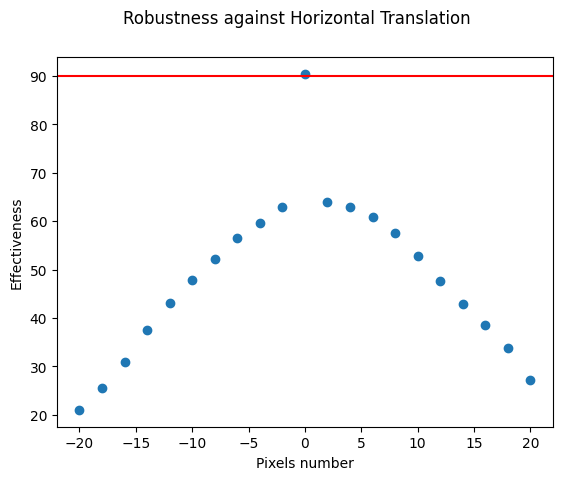
\includegraphics[width=0.9\linewidth]{ImageFiles/EvalBNN/HT/EU/eff}
		\caption{Effectiveness using \\ epistemic uncertainty}
		\label{fig:ht_eu_eff}
	\end{subfigure}
	\caption{Robustness graph for horizontal translation when epistemic uncertainty is employed in the classification}
	\label{fig:ht_eu}
\end{figure}

\Tab~\ref{table:rob_ht_eu} displays the robustness metrics calculated through the utilization of epistemic uncertainty within the classification procedure. The results obtained resemble those from the previous scenario, which confirms the network inherent structural limitations.

\begin{table}[h]
	\centering
	\begin{tabular}{|| l | l ||} 
		\hline
		\textbf{Parameter} & \textbf{Value} \\
		\hline
		\hline
		$rob_{HorizontalTranslation}$ & $0.8933$ \\
		$robInd_{HorizontalTranslation}$ & $0.9001$ \\
		$robAug_{HorizontalTranslation}$ & $0.7752$ \\	
		\hline
	\end{tabular}	
	\caption{Robustness metrics for the horizontal translation when the epistemic uncertainty is employed}
	\label{table:rob_ht_eu}
\end{table}

\vspace{0.3cm}
\textbf{Classification using standard deviation}
\vspace{0.1cm}

The outcomes when employing standard deviation, as illustrated in \Fig~\ref{fig:ht_vu}, do not significantly enhance performance. While there is a slight improvement in accuracy, as shown in \Fig~\ref{fig:ht_vu_acc}, this is counterbalanced by an elevated unknown ratio, as indicated in \Fig~\ref{fig:ht_vu_unkn}, resulting in a similar trend in effectiveness to the previous cases, as seen in \Fig~\ref{fig:ht_vu_eff}.

\begin{figure}[h]
	\centering
	\begin{subfigure}{.33\textwidth}
		\centering
		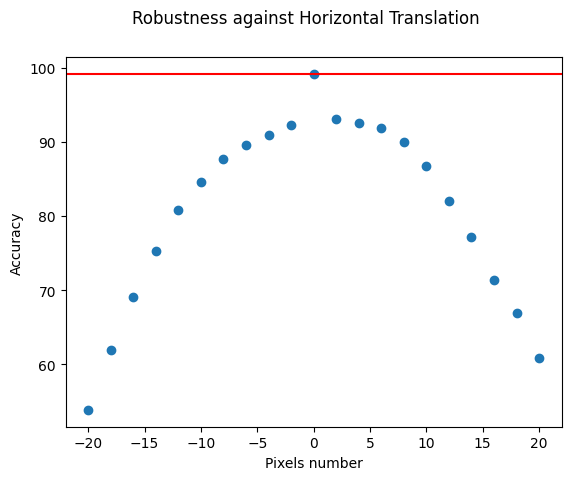
\includegraphics[width=0.9\linewidth]{ImageFiles/EvalBNN/HT/VU/acc}
		\caption{Accuracy using standard \\ deviation}
		\label{fig:ht_vu_acc}
	\end{subfigure}%
	\begin{subfigure}{.33\textwidth}
		\centering
		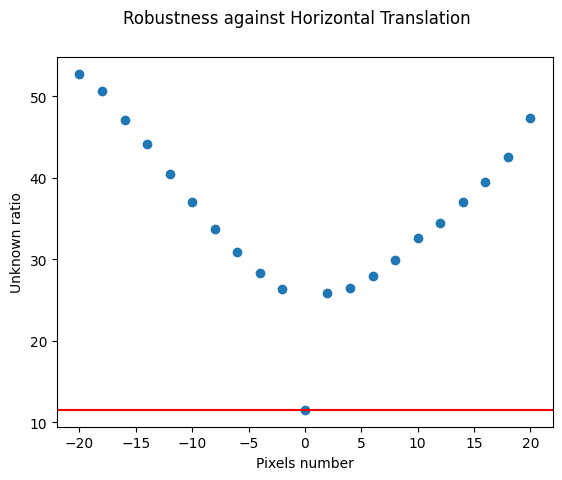
\includegraphics[width=0.9\linewidth]{ImageFiles/EvalBNN/HT/VU/unkn}
		\caption{Unknown ratio using \\ standard deviation}
		\label{fig:ht_vu_unkn}
	\end{subfigure}%
	\begin{subfigure}{.33\textwidth}
		\centering
		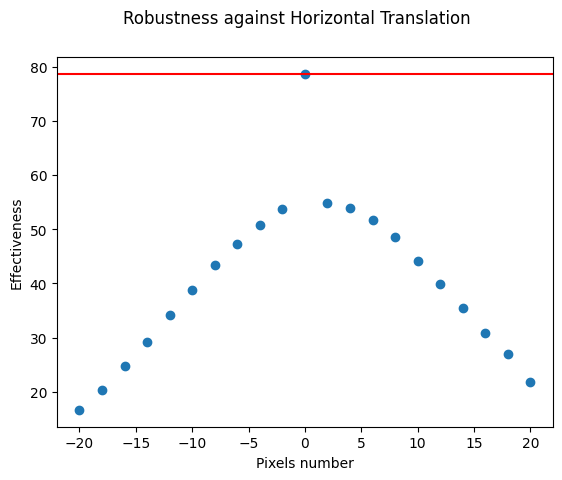
\includegraphics[width=0.9\linewidth]{ImageFiles/EvalBNN/HT/VU/eff}
		\caption{Effectiveness using standard deviation}
		\label{fig:ht_vu_eff}
	\end{subfigure}
	\caption{Robustness graph for horizontal translation when standard deviation is employed in the classification}
	\label{fig:ht_vu}
\end{figure}

\Tab~\ref{table:rob_ht_vu} gives the quantitative robustness metrics.

\begin{table}[h]
	\centering
	\begin{tabular}{|| l | l ||} 
		\hline
		\textbf{Parameter} & \textbf{Value} \\
		\hline
		\hline
		$rob_{HorizontalTranslation}$ & $0.9138$ \\
		$robInd_{HorizontalTranslation}$ & $0.8683$ \\
		$robAug_{HorizontalTranslation}$ & $0.7630$ \\	
		\hline
	\end{tabular}	
	\caption{Robustness metrics for the horizontal translation when the standard deviation is employed}
	\label{table:rob_ht_vu}
\end{table}

\vspace{0.3cm}
\textbf{Comparison}
\vspace{0.1cm}

\Tab~\ref{table:rob_ht} provides an overview of the robustness metrics calculated using various classification methods. It becomes evident that the utilization of uncertainty does not yield a significant improvement, as the network structural limitations continue to play a substantial role.

\begin{table}[h]
	\centering
	\begin{tabular}{|| l | l | l | l ||} 
		\hline
		\textbf{Parameter} & \textbf{Aleatoric} & \textbf{Epistemic} & \textbf{Standard deviation} \\
		\hline
		\hline
		$rob_{HorizontalTranslation}$ & $0.8985$ & $0.8933$ & $0.9138$ \\
		$robInd_{HorizontalTranslation}$ & $0.8993$ & $0.9001$ & $0.8683$ \\
		$robAug_{HorizontalTranslation}$ & $0.7791$ & $0.7752$ & $0.7630$ \\	
		\hline
	\end{tabular}	
	\caption{Summary of the robustness metrics for the horizontal translation}
	\label{table:rob_ht}
\end{table}